% Actividad 2 contractualizada por AulaTeX: mapa conceptual.
\providecommand{\itescastudentname}{Martin Jonathan de la Cruz}
\providecommand{\itescastudentid}{26130503}
\providecommand{\itescastudentemail}{26130503@cajeme.tecnm.mx}
\providecommand{\itescafaculty}{Maestría en Gestión Administrativa}
\providecommand{\itescacoursename}{Fundamentos de Gestión Administrativa}
\providecommand{\itescacoursecode}{ACF--0901}
\providecommand{\itescadepartment}{Posgrado e Investigación}
\providecommand{\itescateachingfigure}{Docente de la materia por confirmar}
\providecommand{\itescaprogramlevel}{Maestría}
\providecommand{\itescaprogramperiod}{Agosto--noviembre de 2026}
\providecommand{\itescamodality}{En línea}
\providecommand{\itescalocation}{Cajeme, Sonora}
\providecommand{\itescaasset}{ITESCA/assets-itesca/itesca-monograma.png}
\providecommand{\itescaofficialasset}{ITESCA/assets-itesca/web/logo-itesca-contorno.png}
\providecommand{\itescasecondaryasset}{ITESCA/assets-itesca/itesca-monograma.png}

\def\itescadocumenttitle {Enfoques múltiples para comprender las organizaciones}
\def\itescadocumentsubtitle {Marcos, metáforas y perspectiva global}
\def\itescadocumentsubject {Actividad 2 - Fundamentos de Gestión Administrativa}
\def\itescaactivityname {Actividad 2. Mapa conceptual}
\def\itescasessionname {Unidad I}
\def\itescablockname {Fundamentos de Gestión Administrativa}
\def\itescamainproduct {Mapa conceptual}

\documentclass[spanish,letterpaper,oneside]{article}

\def\documenttitle {\itescadocumenttitle}
\def\documentsubtitle {\itescadocumentsubtitle}
\def\documentsubject {\itescadocumentsubject}
\def\documentauthor {\itescastudentname}
\def\coursename {\itescacoursename}
\def\coursecode {\itescacoursecode}
\def\universityname {Instituto Tecnológico Superior de Cajeme}
\def\universityfaculty {\itescafaculty}
\def\universitydepartment {\itescadepartment}
\def\universitydepartmentimage {\itescaofficialasset}
\def\universitydepartmentimagecfg {width=5.2cm}
\def\universitylocation {\itescalocation}

\def\authortable {
  \begin{tabular}{ll}
    \textbf{Alumno:} & \itescastudentname \\
    No. de control: & \itescastudentid \\
    Carrera: & \itescafaculty \\
    Semestre: & \itescaprogramperiod \\
    Asignatura: & \itescacoursename \\
    Docente: & \itescateachingfigure \\
    Modalidad: & \itescamodality \\
    Fecha de entrega: & \today \\
    Lugar: & \universitylocation
  \end{tabular}
}

\input{template}
\usepackage{helvet}
\renewcommand{\familydefault}{\sfdefault}
\usepackage{tikz}
\usetikzlibrary{arrows.meta,positioning}
\setcitestyle{numbers,open={[},close={]}}

\definecolor{itescaRedDark}{HTML}{8F1117}
\definecolor{itescaRed}{HTML}{D70F18}
\definecolor{itescaCharcoal}{HTML}{141414}
\definecolor{itescaPaper}{HTML}{F7F7F7}
\def\portraittitlecolor {itescaRedDark}

\hypersetup{
  pdftitle={\itescadocumenttitle},
  pdfsubject={\itescadocumentsubject},
  pdfauthor={\itescastudentname},
  colorlinks=true,
  linkcolor=itescaRedDark,
  citecolor=itescaRedDark,
  urlcolor=itescaRedDark
}

\begin{document}
\templatePortrait
\templatePagecfg
\onehalfspacing

\begin{abstractd}
\textbf{Objetivo:} Sintetizar los enfoques múltiples del análisis organizacional y explicar cómo los marcos de Bolman y Deal, las metáforas de Morgan y la perspectiva global permiten formular diagnósticos complementarios.

\textbf{Producto:} Mapa conceptual jerárquico con conceptos, palabras enlace, proposiciones y relaciones cruzadas.

\textbf{Técnica didáctica:} Mapa conceptual orientado a seleccionar, jerarquizar y relacionar conceptos para representar una explicación integrada.

\textbf{Criterios de entrega:} Cobertura de los enfoques solicitados, claridad jerárquica, relaciones conceptuales legibles, sustento académico y entrega final en PDF.
\end{abstractd}

\templateIndex
\templateFinalcfg

% Técnica didáctica: mapa conceptual.
% Nivel cognitivo: sintetizar y relacionar.
% Criterio de organización: enfoque múltiple -> autores -> lentes -> implicaciones -> entorno global.
\section{Introducción}

Las organizaciones concentran estructuras formales, necesidades humanas, disputas de poder, significados compartidos y presiones del entorno. Ninguna dimensión explica por sí sola por qué una decisión funciona en una institución y fracasa en otra. Bolman y Deal ordenan esa pluralidad en cuatro marcos ---estructural, recursos humanos, político y simbólico--- \citep{bolmanDeal2021}. Morgan muestra, mediante metáforas, que cada lente hace visibles ciertos rasgos y oculta otros \citep{morgan2006}. El mapa conceptual integra ambas clasificaciones y presenta la perspectiva global como lectura transversal del ambiente, no como una equivalencia artificial.

\section{Enfoques múltiples del análisis organizacional}

\subsection{Preparación conceptual}

El \textbf{marco estructural} estudia roles, reglas, metas y coordinación; el de \textbf{recursos humanos}, el ajuste entre personas y organización; el \textbf{político}, los intereses, coaliciones, conflictos y recursos escasos; y el \textbf{simbólico}, la cultura, los rituales, relatos y significados \citep{bolmanDeal2021}. Las metáforas de máquina, organismo, cerebro, cultura, sistema político, prisión psíquica, flujo y transformación, e instrumento de dominación ofrecen imágenes críticas complementarias \citep{morgan2006}. La \textbf{perspectiva global} incorpora fuerzas económicas, tecnológicas, político-legales, socioculturales y ambientales que condicionan todas las dimensiones internas \citep{bright2019,openstaxEnvironment2019}.

\begin{landscape}
\thispagestyle{empty}
\begingroup
\centering
\resizebox{0.97\linewidth}{!}{%
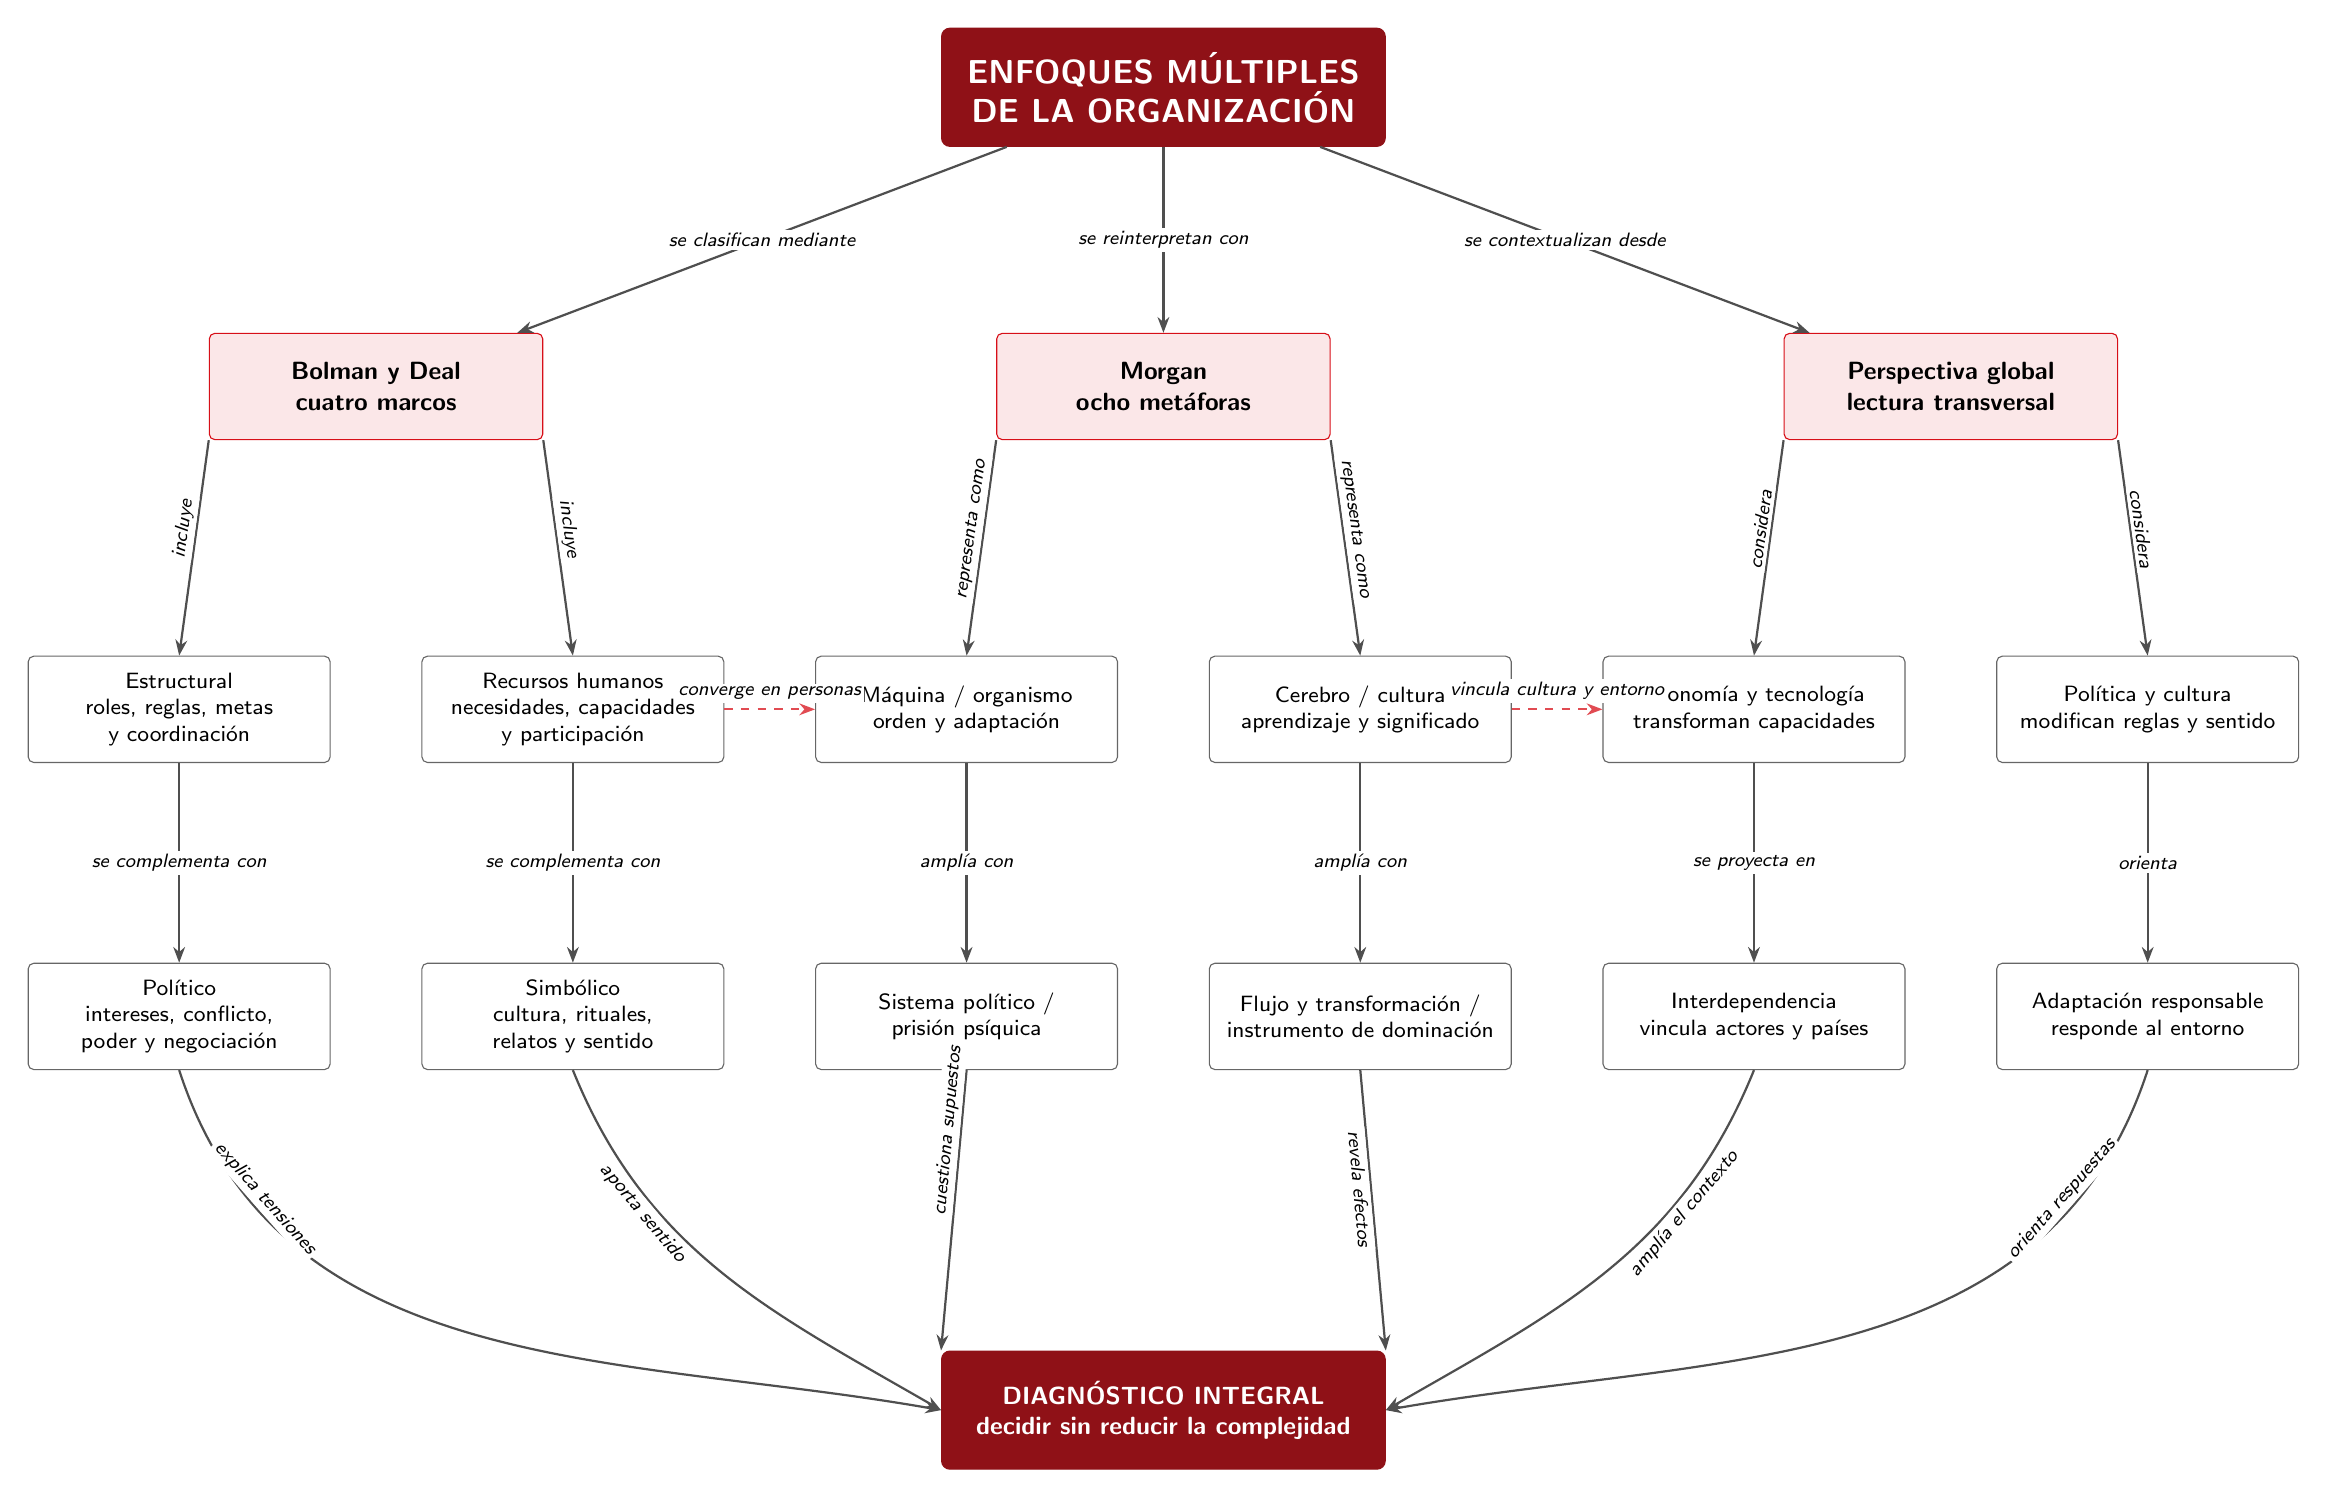
\begin{tikzpicture}[
 root/.style={rounded corners=3pt,draw=itescaRedDark,fill=itescaRedDark,text=white,font=\bfseries\large,align=center,text width=5.4cm,minimum height=1.5cm},
 branch/.style={rounded corners=2pt,draw=itescaRed,fill=itescaRed!10,font=\bfseries\small,align=center,text width=4cm,minimum height=1.35cm},
 concept/.style={rounded corners=2pt,draw=itescaCharcoal!65,fill=white,font=\footnotesize,align=center,text width=3.6cm,minimum height=1.35cm},
 edge/.style={-{Stealth[length=2mm]},thick,draw=itescaCharcoal!75},
 cross/.style={-{Stealth[length=2mm]},thick,dashed,draw=itescaRed!75},
 label/.style={font=\scriptsize\itshape,fill=white,inner sep=1.2pt,align=center}
]
\node[root] (root) at (0,15.6) {ENFOQUES MÚLTIPLES\\DE LA ORGANIZACIÓN};
\node[branch] (bd) at (-10,11.8) {Bolman y Deal\\cuatro marcos};
\node[branch] (mo) at (0,11.8) {Morgan\\ocho metáforas};
\node[branch] (gl) at (10,11.8) {Perspectiva global\\lectura transversal};
\draw[edge] (root) -- node[label]{se clasifican mediante} (bd);
\draw[edge] (root) -- node[label]{se reinterpretan con} (mo);
\draw[edge] (root) -- node[label]{se contextualizan desde} (gl);

\node[concept] (es) at (-12.5,7.7) {Estructural\\roles, reglas, metas\\y coordinación};
\node[concept] (rh) at (-7.5,7.7) {Recursos humanos\\necesidades, capacidades\\y participación};
\node[concept] (po) at (-12.5,3.8) {Político\\intereses, conflicto,\\poder y negociación};
\node[concept] (si) at (-7.5,3.8) {Simbólico\\cultura, rituales,\\relatos y sentido};
\draw[edge] (bd.south west) -- node[label,pos=.42,sloped,above]{incluye} (es.north);
\draw[edge] (bd.south east) -- node[label,pos=.42,sloped,above]{incluye} (rh.north);
\draw[edge] (es.south) -- node[label,pos=.50,fill=white]{se complementa con} (po.north);
\draw[edge] (rh.south) -- node[label,pos=.50,fill=white]{se complementa con} (si.north);

\node[concept] (m1) at (-2.5,7.7) {Máquina / organismo\\orden y adaptación};
\node[concept] (m2) at (2.5,7.7) {Cerebro / cultura\\aprendizaje y significado};
\node[concept] (m3) at (-2.5,3.8) {Sistema político /\\prisión psíquica};
\node[concept] (m4) at (2.5,3.8) {Flujo y transformación /\\instrumento de dominación};
\draw[edge] (mo.south west) -- node[label,pos=.42,sloped,above]{representa como} (m1.north);
\draw[edge] (mo.south east) -- node[label,pos=.42,sloped,above]{representa como} (m2.north);
\draw[edge] (m1.south) -- node[label,pos=.50,fill=white]{amplía con} (m3.north);
\draw[edge] (m2.south) -- node[label,pos=.50,fill=white]{amplía con} (m4.north);

\node[concept] (g1) at (7.5,7.7) {Economía y tecnología\\transforman capacidades};
\node[concept] (g2) at (12.5,7.7) {Política y cultura\\modifican reglas y sentido};
\node[concept] (g3) at (7.5,3.8) {Interdependencia\\vincula actores y países};
\node[concept] (g4) at (12.5,3.8) {Adaptación responsable\\responde al entorno};
\draw[edge] (gl.south west) -- node[label,pos=.42,sloped,above]{considera} (g1.north);
\draw[edge] (gl.south east) -- node[label,pos=.42,sloped,above]{considera} (g2.north);
\draw[edge] (g1.south) -- node[label,pos=.50,fill=white]{se proyecta en} (g3.north);
\draw[edge] (g2.south) -- node[label,pos=.50,fill=white]{orienta} (g4.north);

\node[root,font=\bfseries\small,minimum width=5.5cm] (diag) at (0,-1.2) {DIAGNÓSTICO INTEGRAL\\decidir sin reducir la complejidad};
\draw[edge] (po.south) to[out=-72,in=170] node[label,pos=.18,sloped,above]{explica tensiones} (diag.west);
\draw[edge] (si.south) to[out=-68,in=150] node[label,pos=.30,sloped,below]{aporta sentido} (diag.west);
\draw[edge] (m3.south) -- node[label,pos=.22,sloped,above]{cuestiona supuestos} (diag.north west);
\draw[edge] (m4.south) -- node[label,pos=.42,sloped,below]{revela efectos} (diag.north east);
\draw[edge] (g3.south) to[out=-112,in=30] node[label,pos=.30,sloped,below]{amplía el contexto} (diag.east);
\draw[edge] (g4.south) to[out=-108,in=10] node[label,pos=.18,sloped,above]{orienta respuestas} (diag.east);

\draw[cross] (rh.east) -- node[label,pos=.50,above=2pt]{converge en personas} (m1.west);
\draw[cross] (m2.east) -- node[label,pos=.50,above=2pt]{vincula cultura y entorno} (g1.west);
\end{tikzpicture}}

\par\vspace{0.03cm}
\begin{minipage}{0.88\linewidth}
\centering\scriptsize
\textbf{Figura 1.} Los marcos de acción, las metáforas interpretativas y las condiciones globales convergen en un diagnóstico integral. Elaboración propia con base en \citeauthor{bolmanDeal2021}, \citeauthor{morgan2006} y \citeauthor{bright2019}.
\end{minipage}
\endgroup
\end{landscape}

\subsection{Lectura del mapa conceptual}

La primera rama conduce a los cuatro marcos de Bolman y Deal. Desde recursos humanos, una baja productividad puede indicar falta de capacidades, reconocimiento o participación; desde el marco político, el mismo síntoma puede revelar competencia por recursos y desacuerdo entre coaliciones; desde el simbólico, puede expresar pérdida de identidad o legitimidad. El marco estructural pregunta si responsabilidades, reglas y procesos están alineados con la estrategia.

La segunda rama incorpora las metáforas de Morgan como dispositivos críticos. Ver una institución como máquina hace visibles estandarización y control, mientras verla como organismo destaca adaptación y supervivencia. Las imágenes de cultura y sistema político se aproximan a los marcos simbólico y político, pero no son equivalentes: Morgan explora formas de imaginar la organización y Bolman y Deal ordenan perspectivas para comprenderla y actuar sobre ella \citep{bolmanDeal2021,morgan2006}.

La tercera rama muestra que cambios tecnológicos, regulación, diversidad cultural, mercados y problemas ambientales alteran competencias, estructuras, poder y significados. La perspectiva global obliga a volver sobre todas las ramas y preguntar cómo una decisión local depende de actores y fuerzas externas \citep{openstaxEnvironment2019}. El diagnóstico integral surge de contrastar lentes y seleccionar una respuesta congruente con personas, intereses, símbolos, diseño y entorno.

\clearpage
\section{Conclusiones}

Los enfoques múltiples impiden confundir una explicación parcial con la organización completa. Bolman y Deal ofrecen cuatro marcos accionables; Morgan demuestra que toda imagen ilumina ciertos procesos y oscurece otros; y la perspectiva global recuerda que las fronteras organizacionales son permeables. Mi postura es que un diagnóstico responsable debe comenzar con el marco que mejor explique el problema, contrastarlo al menos con otro y revisar después las presiones externas. Esta secuencia reduce decisiones mecánicas: una reestructuración puede requerir simultáneamente nuevas capacidades, negociación política y reconstrucción de significado. El mapa convierte esa pluralidad teórica en una guía de análisis aplicable.\footnote{Declaración de uso: se utilizó inteligencia artificial como apoyo para organizar, revisar y editar el texto y el diagrama; el autor verificó las fuentes, asumió la postura expresada y conserva la responsabilidad sobre el contenido final.}

\clearpage
\begin{thebibliography}{9}

\bibitem[Bolman y Deal(2021)]{bolmanDeal2021}
Bolman, L. G. y Deal, T. E. (2021).
\textit{Reframing Organizations: Artistry, Choice, and Leadership} (7.ª ed.).
Jossey-Bass. \url{https://www.wiley.com/en-us/Reframing+Organizations%3A+Artistry%2C+Choice%2C+and+Leadership%2C+7th+Edition-p-9781119756835}

\bibitem[Morgan(2006)]{morgan2006}
Morgan, G. (2006).
\textit{Images of Organization} (edición actualizada).
SAGE Publications. \url{https://us.sagepub.com/en-us/nam/images-of-organization/book252708}

\bibitem[Bright et al.(2019)]{bright2019}
Bright, D. S. y Cortes, A. H. (eds.). (2019).
\textit{Principles of Management}.
OpenStax, Rice University. \url{https://openstax.org/details/books/principles-management}

\bibitem[Weiss(2019)]{openstaxEnvironment2019}
Weiss, J. W. (2019).
The Organization's External Environment.
En \textit{Principles of Management}. OpenStax, Rice University.
\url{https://openstax.org/books/principles-management/pages/4-1-the-organizations-external-environment}

\end{thebibliography}

\end{document}
